\documentclass[border=6pt]{standalone}
\usepackage{tikz}
\usepackage[edges]{forest}
\usetikzlibrary{arrows.meta,positioning,calc,decorations.pathreplacing,shapes.geometric}
\begin{document}
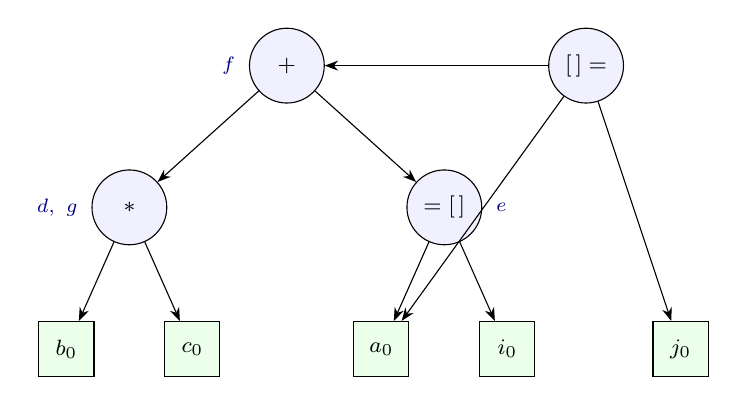
\begin{tikzpicture}[>=Stealth,font=\small,
 op/.style={draw,circle,minimum size=0.95cm,inner sep=0pt,fill=blue!6,font=\footnotesize},
 lf/.style={draw,rectangle,minimum size=0.7cm,inner sep=2pt,fill=green!8,font=\footnotesize},
 lb/.style={font=\scriptsize,blue!50!black}]
\node[lf] (b0) at (0,0) {$b_0$}; \node[lf] (c0) at (1.6,0) {$c_0$};
\node[lf] (a0) at (4.0,0) {$a_0$}; \node[lf] (i0) at (5.6,0) {$i_0$}; \node[lf] (j0) at (7.8,0) {$j_0$};
\node[op] (n1) at (0.8,1.8) {$*$}; \node[lb,left=0.05cm of n1] {$d,\ g$};
\node[op] (n2) at (4.8,1.8) {$=[\,]$}; \node[lb,right=0.05cm of n2] {$e$};
\node[op] (n3) at (2.8,3.6) {$+$}; \node[lb,left=0.05cm of n3] {$f$};
\node[op] (n4) at (6.6,3.6) {$[\,]=$};
\draw[->] (n1)--(b0); \draw[->] (n1)--(c0);
\draw[->] (n2)--(a0); \draw[->] (n2)--(i0);
\draw[->] (n3)--(n2); \draw[->] (n3)--(n1);
\draw[->] (n4)--(a0); \draw[->] (n4)--(j0); \draw[->] (n4)--(n3);
\end{tikzpicture}
\end{document}
